\section{Experiments and discussion}
\label{sec:experiments}

% Experimental setup
The simulations had 100 agents interacting over 21 virtual days, initialized with profiles, personalities and opinions.
The model used is \textit{artifish/llama3.2-uncensored}, available on \textit{Ollama}, chosen for its lack of filters, essential when dealing with political topics or controversial opinions.

Different scenarios were tested by varying two parameters: the level of misinformation (0\%, 5\%, 10\%, and 50\%), and the content recommendation system.
Specifically, two recommender algorithms were used:
\begin{itemize}
    \item \textit{ReverseChronoFollowersPopularity}, which shows recent posts from followed users, with some content from non-followed users to ensure exposure to different views
    \item \textit{ContentRecSys}, suggesting random content
\end{itemize}

Each scenario was run 10 to 20 times with new agents, to ensure the robustness of the results.



% Results and discussion
\medskip
The analysis is structured on multiple levels to provide a overview of the behavior of LLMs agents within a simulated social media.

% Interactions
\subsection{Interactions}

% Activity per user type + network structure
The comparison of interaction activity by user type, in Figure \ref{fig:interactions_count}, shows that misinformation agents are more active in content generation, as they post and comment more than base users. However, they engage less in building connections, as \textit{follows} are significantly lower.
\textit{Likes} are used similarly by the two groups, while base users are more active in expressing disagreement through \textit{dislikes}.
Thanks to the \textit{follow} action, users form connections across coalitions and between different agent types, allowing a structured network to emerge. The \textit{unfollow} action, instead, is almost absent, suggesting that longer simulations may be needed to see a observe the evolution of of connections over time.

\begin{figure}[h]
    \centering
    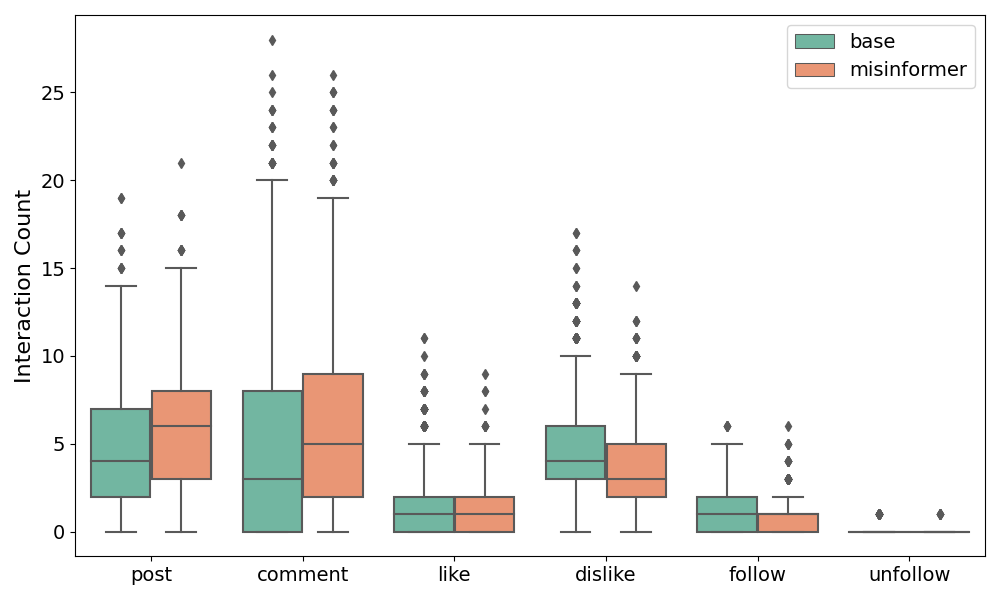
\includegraphics[width=1\linewidth]{Images/Interactions/count_per_user_DefaultRecSys.png}
    \caption{Number of interactions per user by agent type.}
    \label{fig:interactions_count}
\end{figure}

% In-group and out-group interactions across coalitions
\medskip
To analyze how users interact within and across coalitions, Figure \ref{fig:interactions_inout} shows, for each coalition, the percentage of in-group interactions, categorizing the actions into positive (\textit{like}, \textit{follow}) and negative (\textit{dislike}, \textit{unfollow}).

Looking at positive interactions, Centre-Left and Third Pole show a balanced behavior, with about a half of their \textit{likes} and \textit{follows} directed at in-group users.

In contrast, M5S and Right show fewer in-group positive interactions. 
For M5S, this may be due to its smaller size in the simulated populations, which increases the chance of out-group interactions.
The Right, even though it's one of the largest group, still shows a strong preference for out-group positive interactions.

Negative interactions are mostly directed toward other coalitions, and the Right stands out for the higher rate of in-group negative interactions.
This might indicate that the Right may have a greater level of internal fragmentation, with more conflict even among users with the same political views.


\begin{figure}[h]
    \centering
    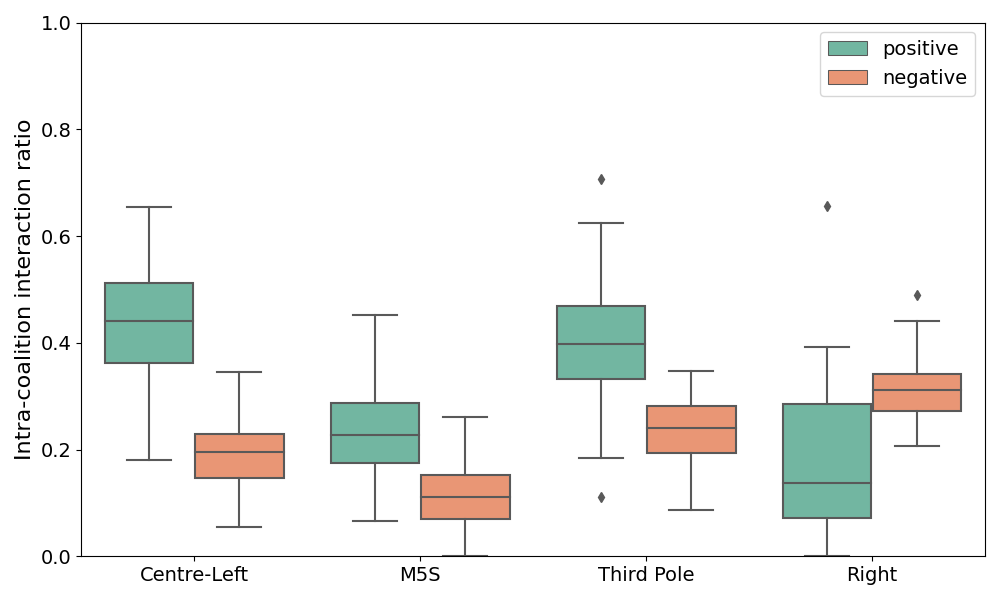
\includegraphics[width=1\linewidth]{Images/Interactions/pos_neg_in_DefaultRecSys.png}
    \caption{Percentage of in-group interactions, divided into positive and negative interactions, for each coalition.}
    \label{fig:interactions_inout}
\end{figure}


% Opinion
\subsection{Opinion evolution}
One important aspect introduced in this work in extension to the existing simulator is opinion modeling.
Figure \ref{fig:opinion_evolution} shows that the opinion evolution of scores assigned by LLMs have the same trends as traditional opinion dynamics models.
This confirms that LLMs can effectively model opinion change at population level.
Coalitions that start with the same opinion tend to evolve in parallel, suggesting that their initial view is more influential than the coalition itself.
Moreover, across all topics, there's a gradual convergence toward neutral values, indicating a general reduction in polarization over time.


\begin{figure}[h]
    \centering
    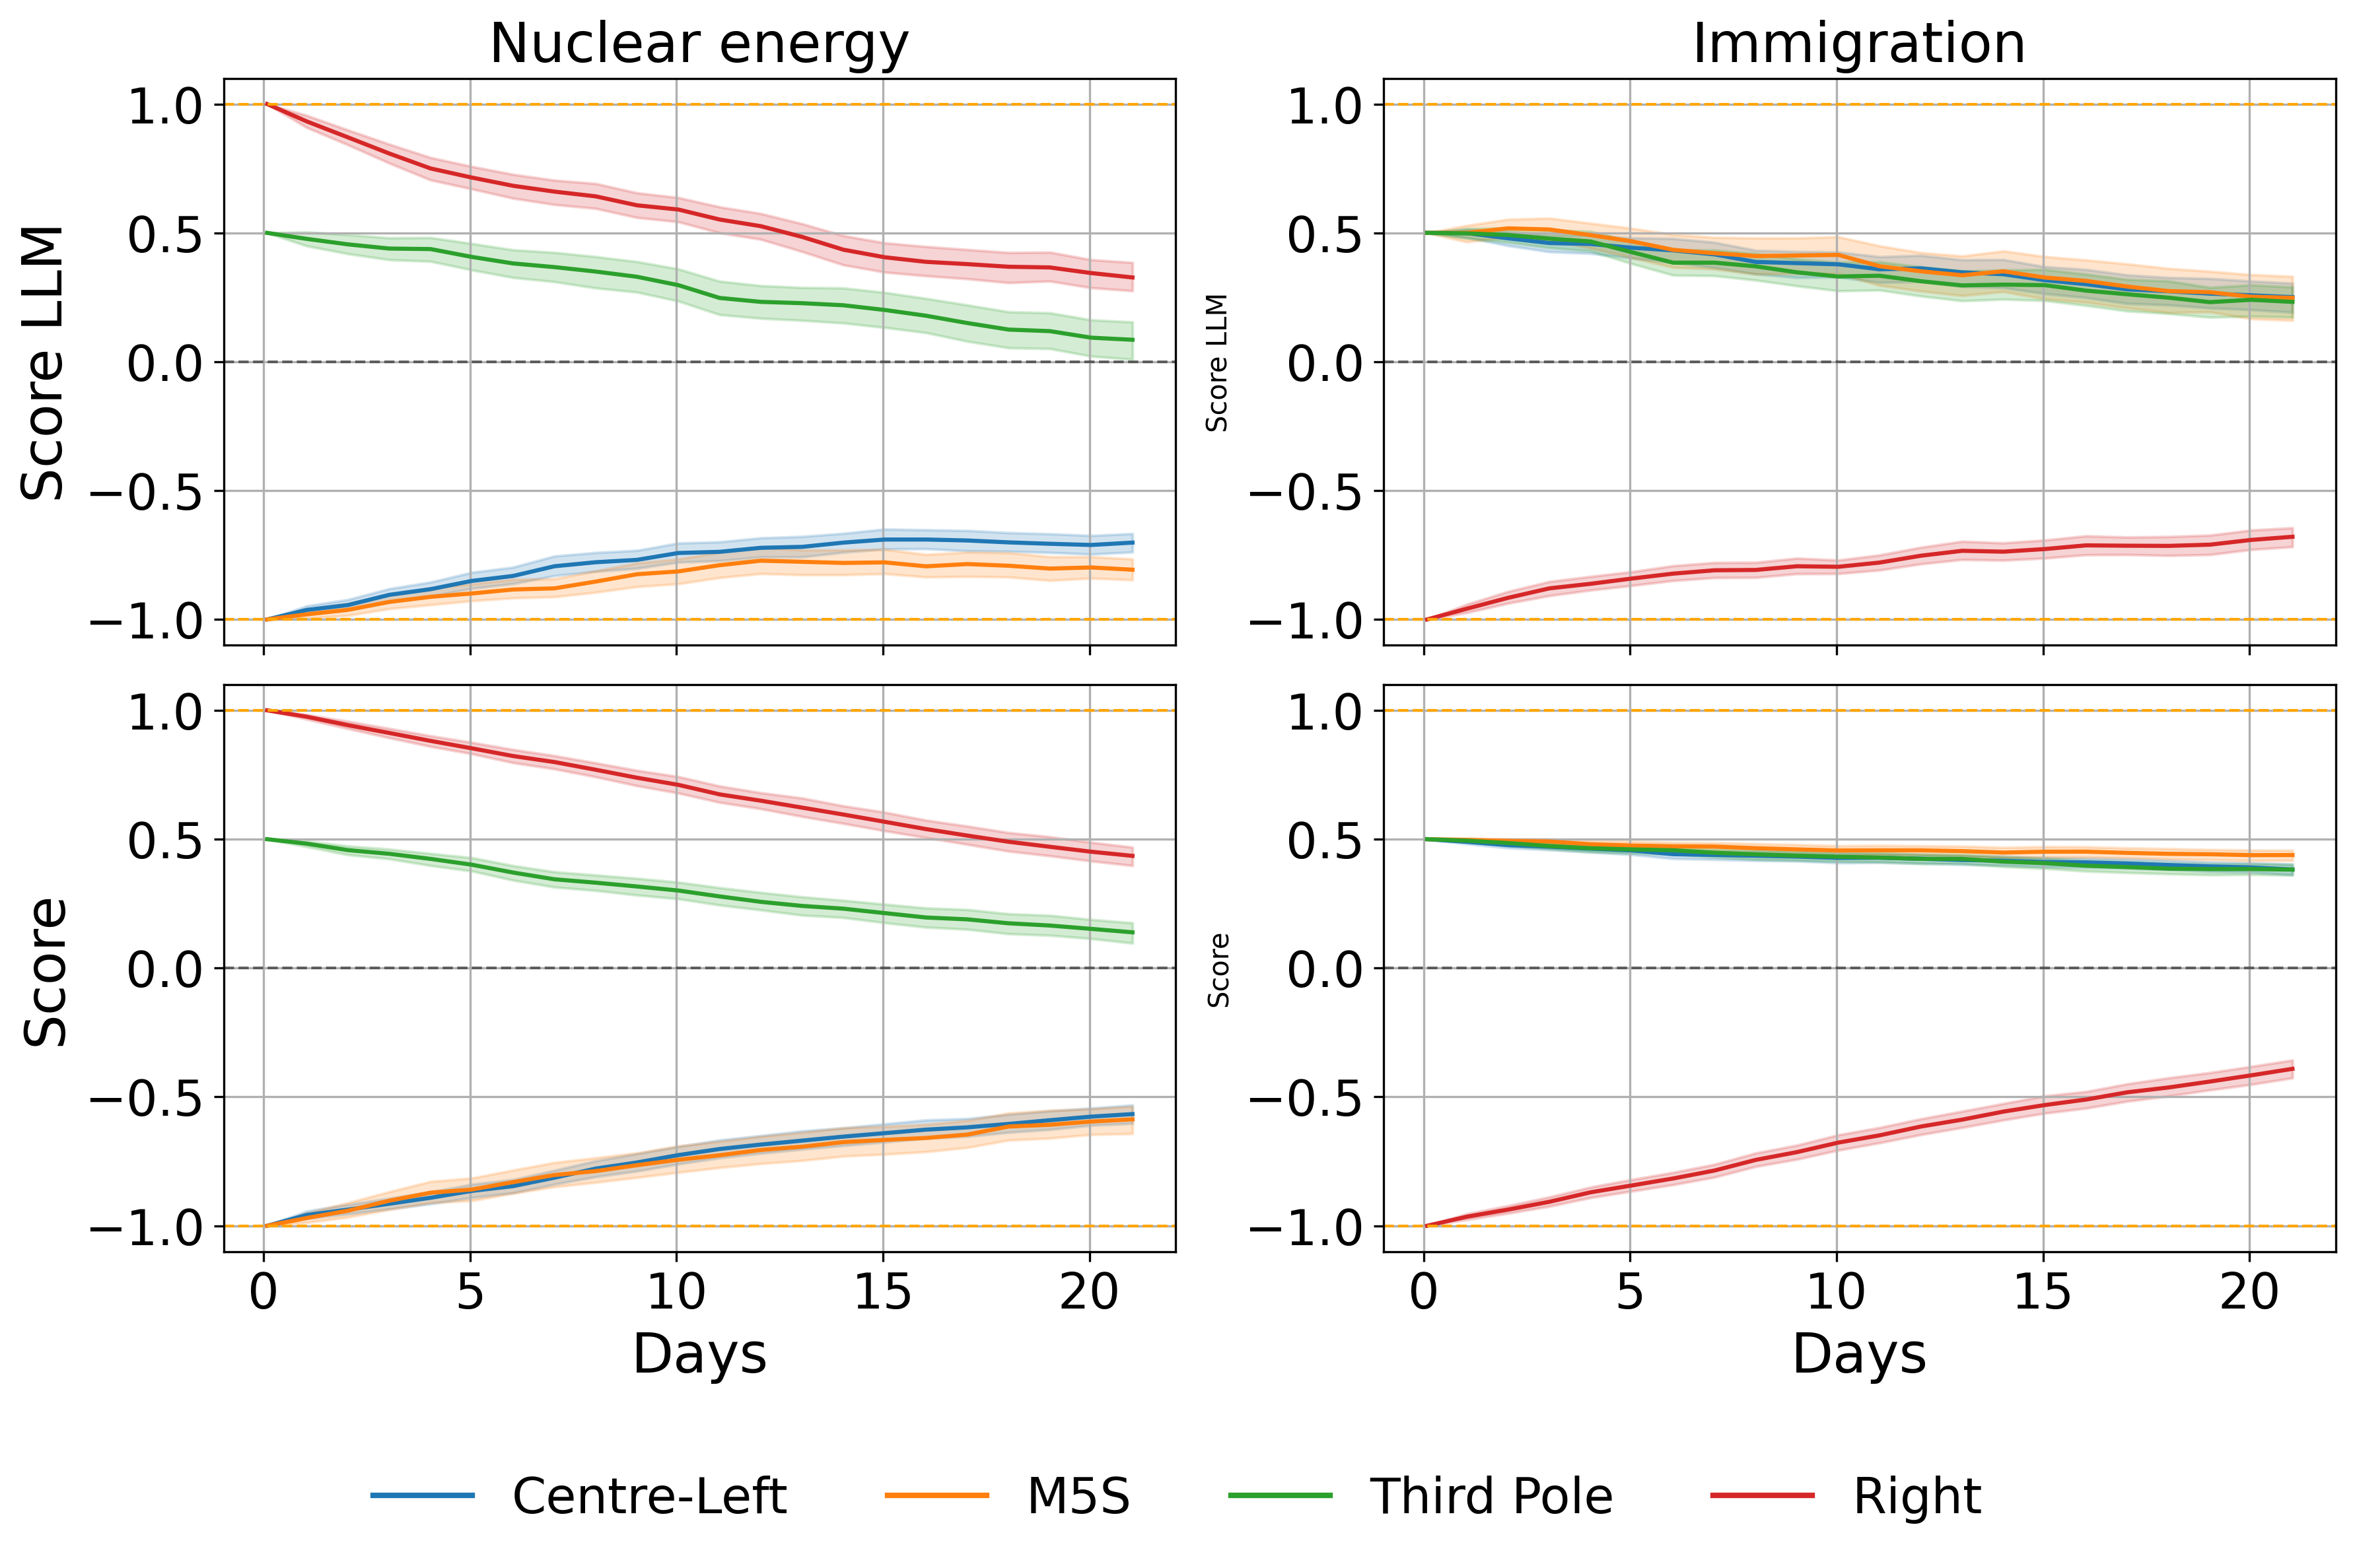
\includegraphics[width=1\linewidth]{Images/Opinions/d21a100m00x_RandomRecSys.png}
    \caption{Opinion evolution, with scores assigned by the LLM and a traditional model.}
    \label{fig:opinion_evolution}
\end{figure}


% Misinformation
\subsection{Misinformation}
To evaluate the impact of misinformation, we considered opinion shift, which is the difference between each user’s final opinion and their initial opinion.
Results in Figure \ref{fig:misinfo_opinion_shift} show that increasing the amount of misinformation in the system doesn’t significantly affect how agents update their views.
Even in the extreme scenario with 50\% of agents producing misleading content, opinion shifts remains similar to those in setups with lower misinformation.

% Confirmation bias
A possible question is whether the lack of misinformation impact might be related to the confirmation bias, which was explicitly introduced in this work.
While the bias is visible, in the narrow distributions indicating a resistance to opinion change, it affects all conditions equally, and doesn't explain the absence of differences across misinformation levels.
Agents do evolve their opinions over time, but the dynamics of change are independent from the misinformation exposure.

% Coalitions
%A comparison between different coalitions highlights that the Right has the narrowest distributions, suggesting greater resistant to change.
%This may be due to their stronger initial stances, both in the numerical scores and in the descriptions of their view, which led agents to remain closer to their starting position.

% Conclusion on LLM limitation
These findings reveal a limitation: even though LLMs can simulate realistic opinion change, they don't replicate the real-world susceptibility to misinformation.
This may be due to missing factors such as emotional reasoning or social signals such as popularity or perceived credibility.
Adding these factors could improve future simulations.


\begin{figure}[h]
    \centering
    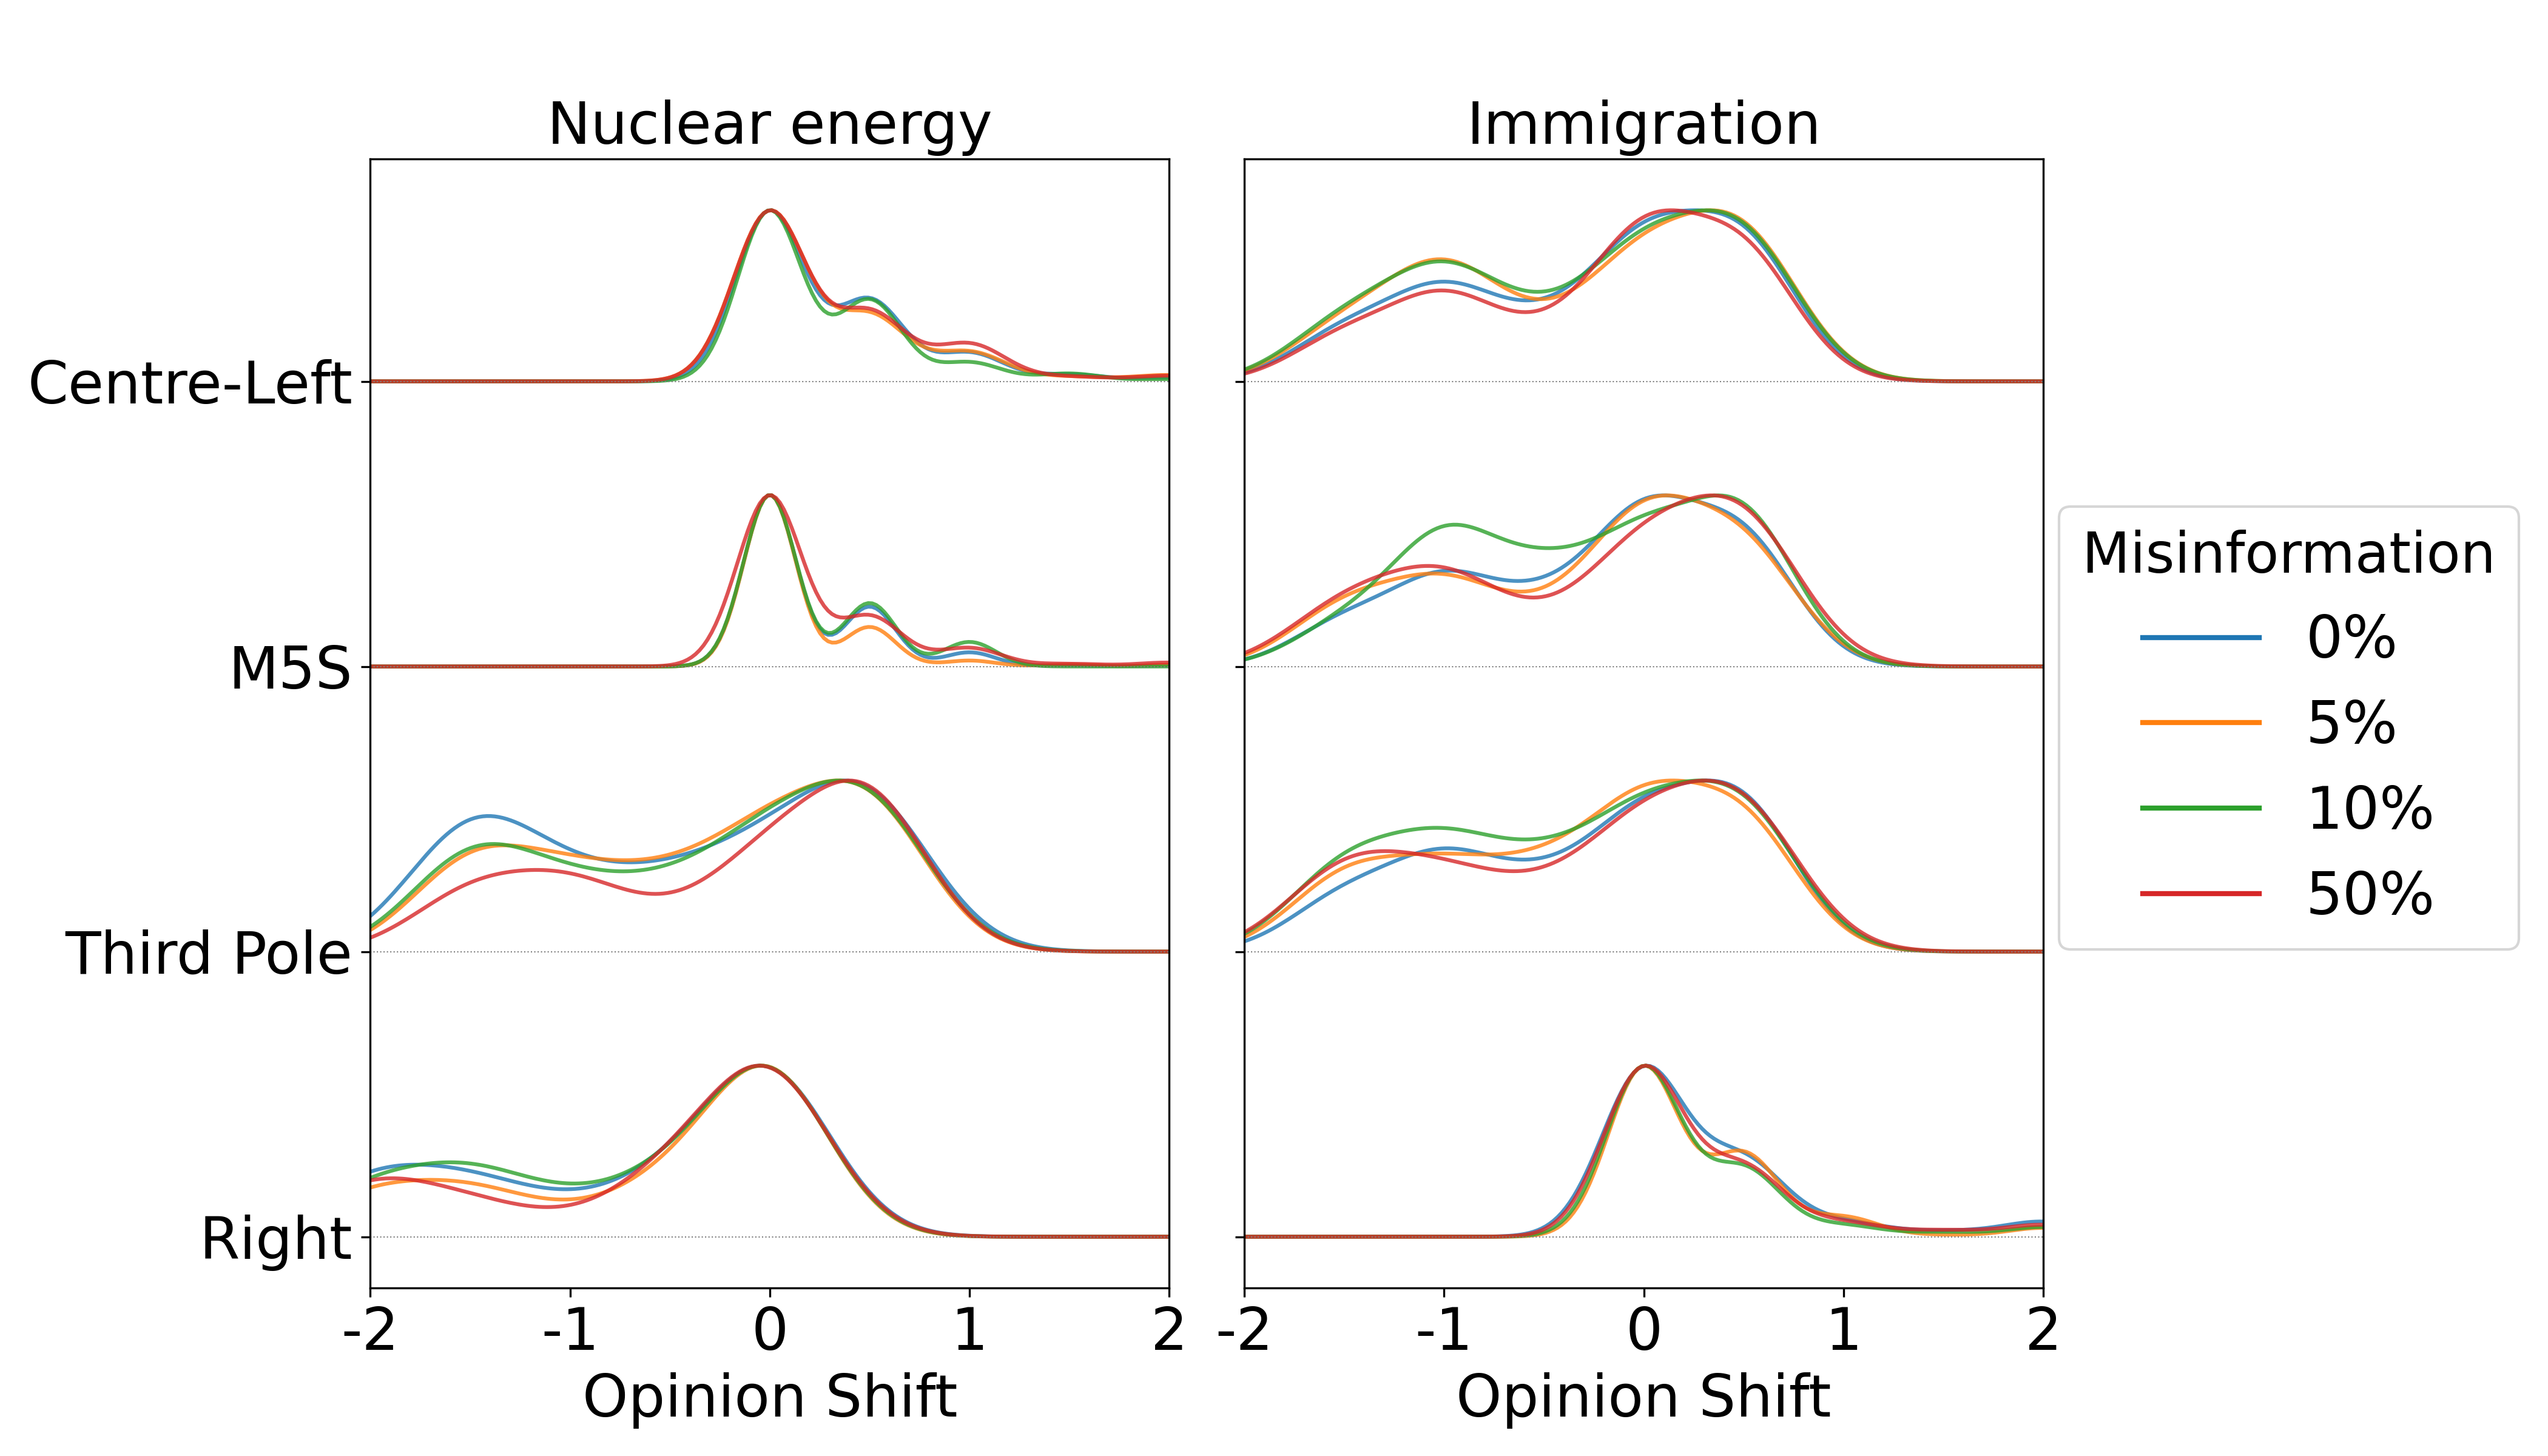
\includegraphics[width=1\linewidth]{Images/Misinformation/score_llm_RandomRecSys_small.png}
    \caption{Distribution of opinion shift (difference between final and initial opinion) for each topic an coalition, with varying levels of misinformation.}
    \label{fig:misinfo_opinion_shift}
\end{figure}


% Toxicity
\subsection{Toxicity analysis}

% Toward in-group and out-group 
To evaluate how agents express toxicity toward different groups, we compute the delta of the toxicity of their comments directed to out-group and in-group users.
Figure \ref{fig:toxicity_in_out} shows the distributions, on a logarithmic scale.
Both real and simulated data are centered around zero, indicating that agents don't have a specific preference in toxicity direction.

However, the real data have a wider distribution, indicating that real users show greater variability in the toxicity toward the two groups.
This suggests that the simulations fail to reproduce the diversity of behavior of real world  in how toxicity is distributed.



\begin{figure}[h]
    \centering
    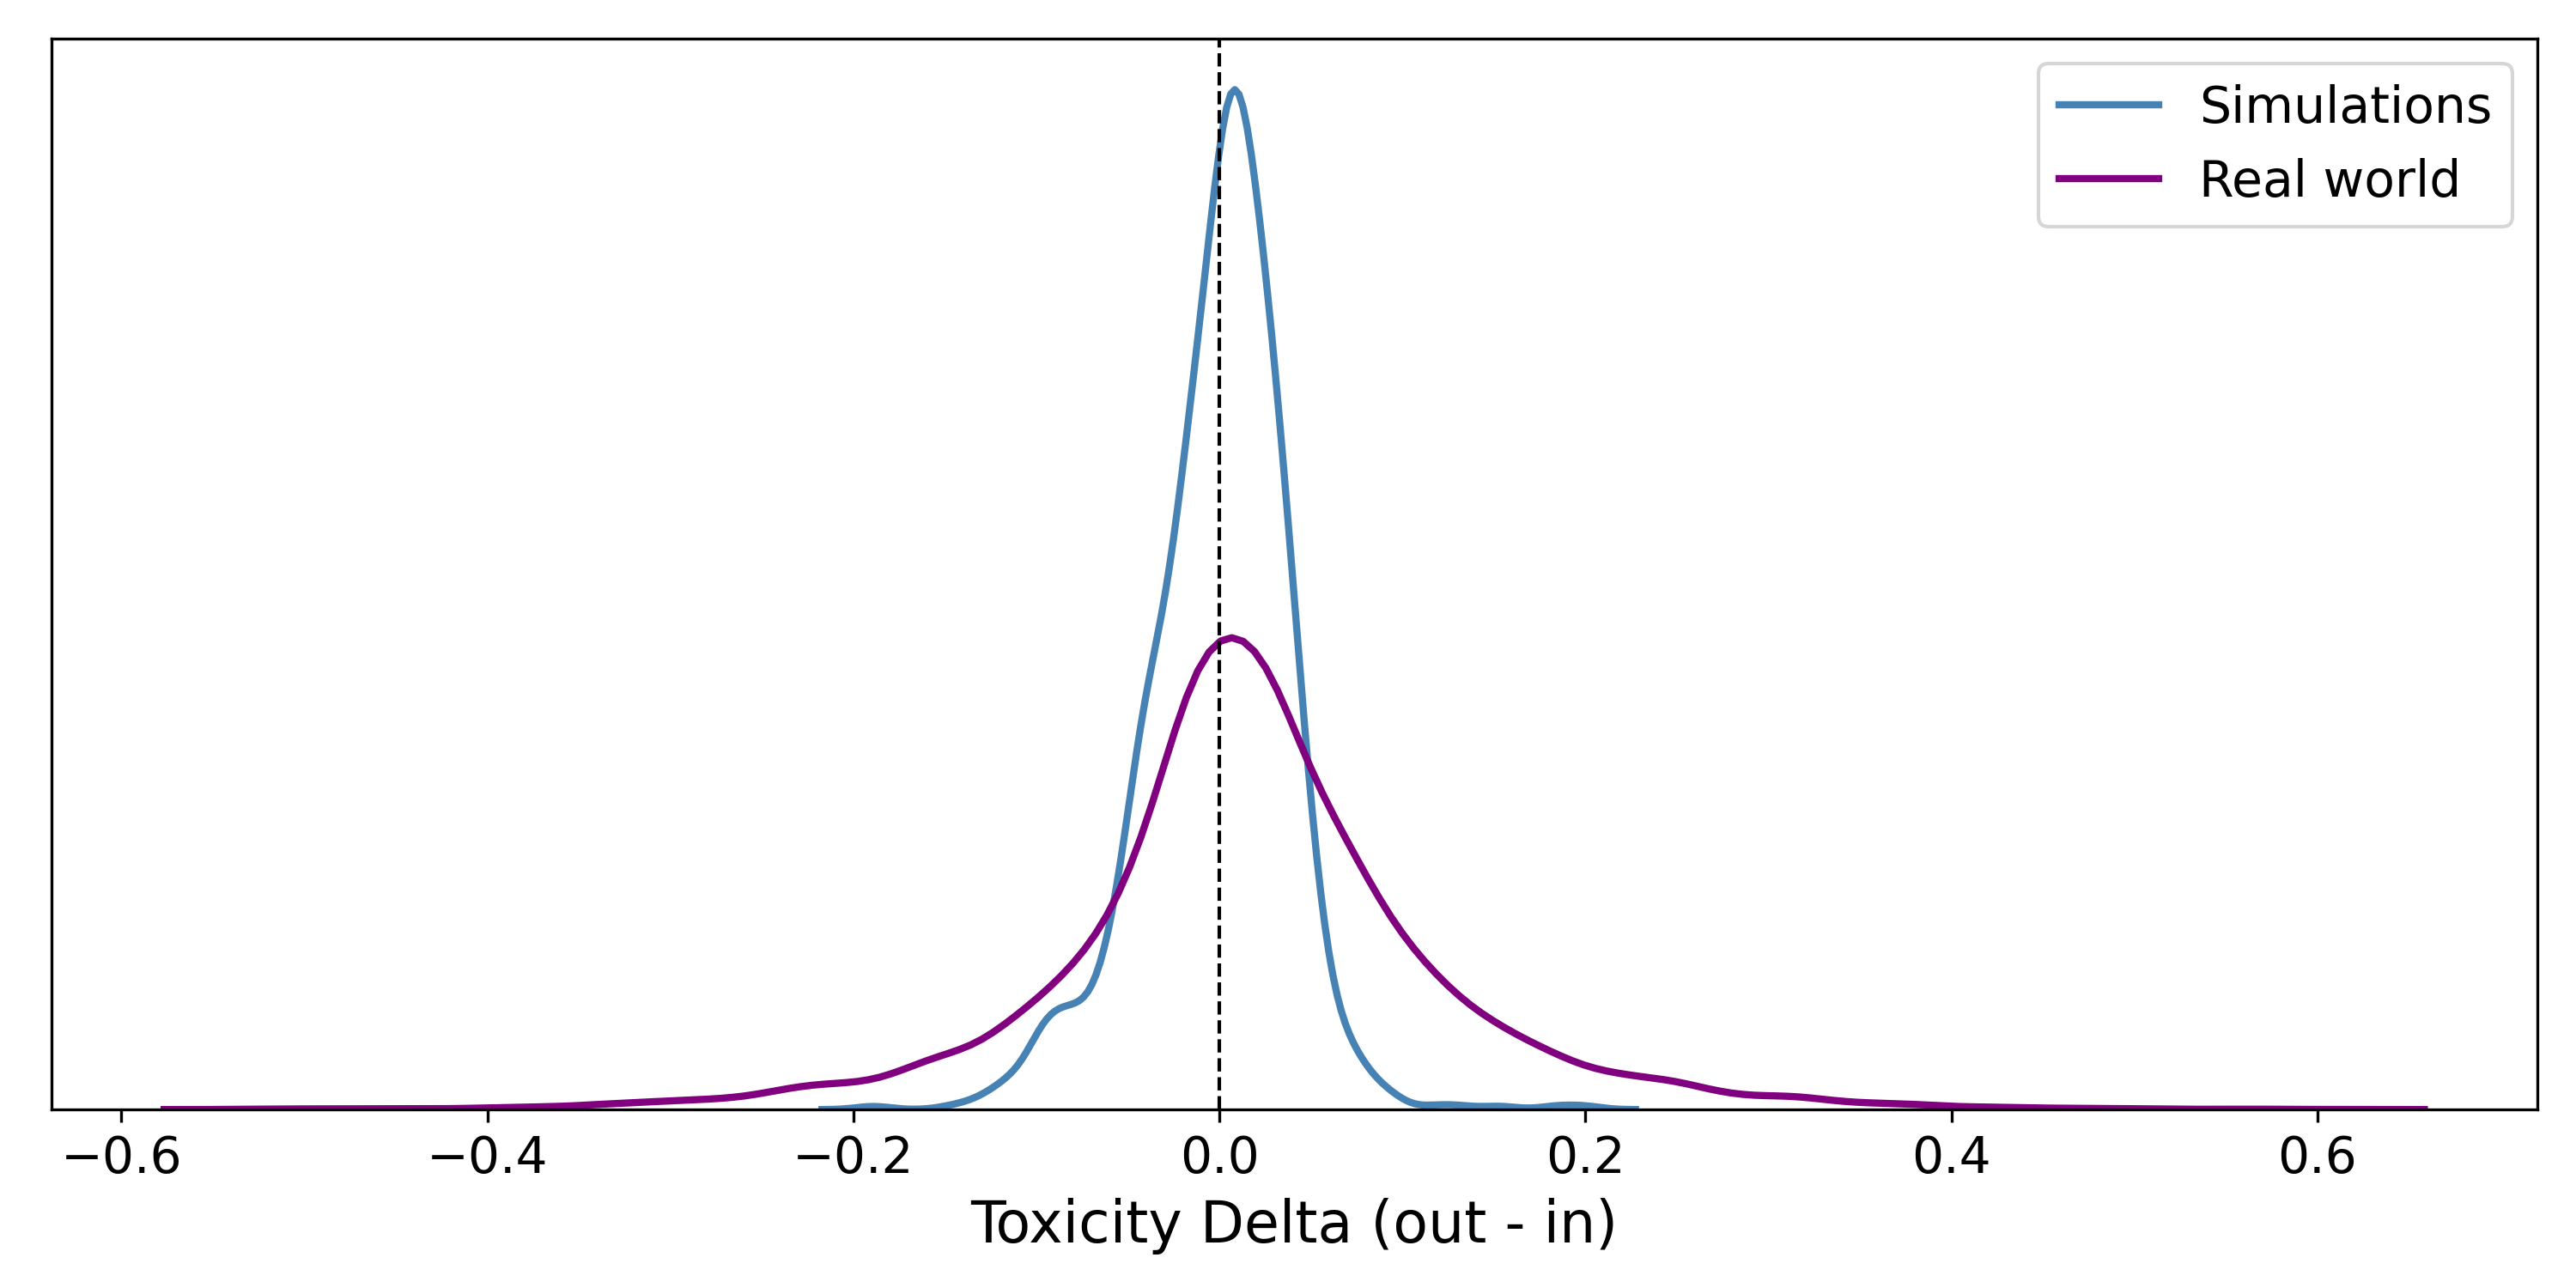
\includegraphics[width=1\linewidth]{Images/Toxicity/diff_in_out_combined.png}
    \caption{Distribution of the difference in mean toxicity toward out-group and in-group in user comments.}
    \label{fig:toxicity_in_out}
\end{figure}


% Across coalitions and content types
\medskip
Figure \ref{fig:toxicity_box} investigates on how toxicity varies across political coalition and content types.

In general, posts tend to be more toxic on average than comments, except for the right coalition, which may indicate a more conflictual style in replying.
M5S has the highest average toxicity in posts, whereas Centre-Left and Third Pole maintain a more moderate and stable tone in both types of contents.

Despite the low average values, all distributions have positive skew, suggesting that LLMs can produce highly toxic content, even though at lower frequency.
This behavior, maybe facilitated by the use of an uncensored model, contributes to a more realistic simulation of online conversations.


\begin{figure}[h]
    \centering
    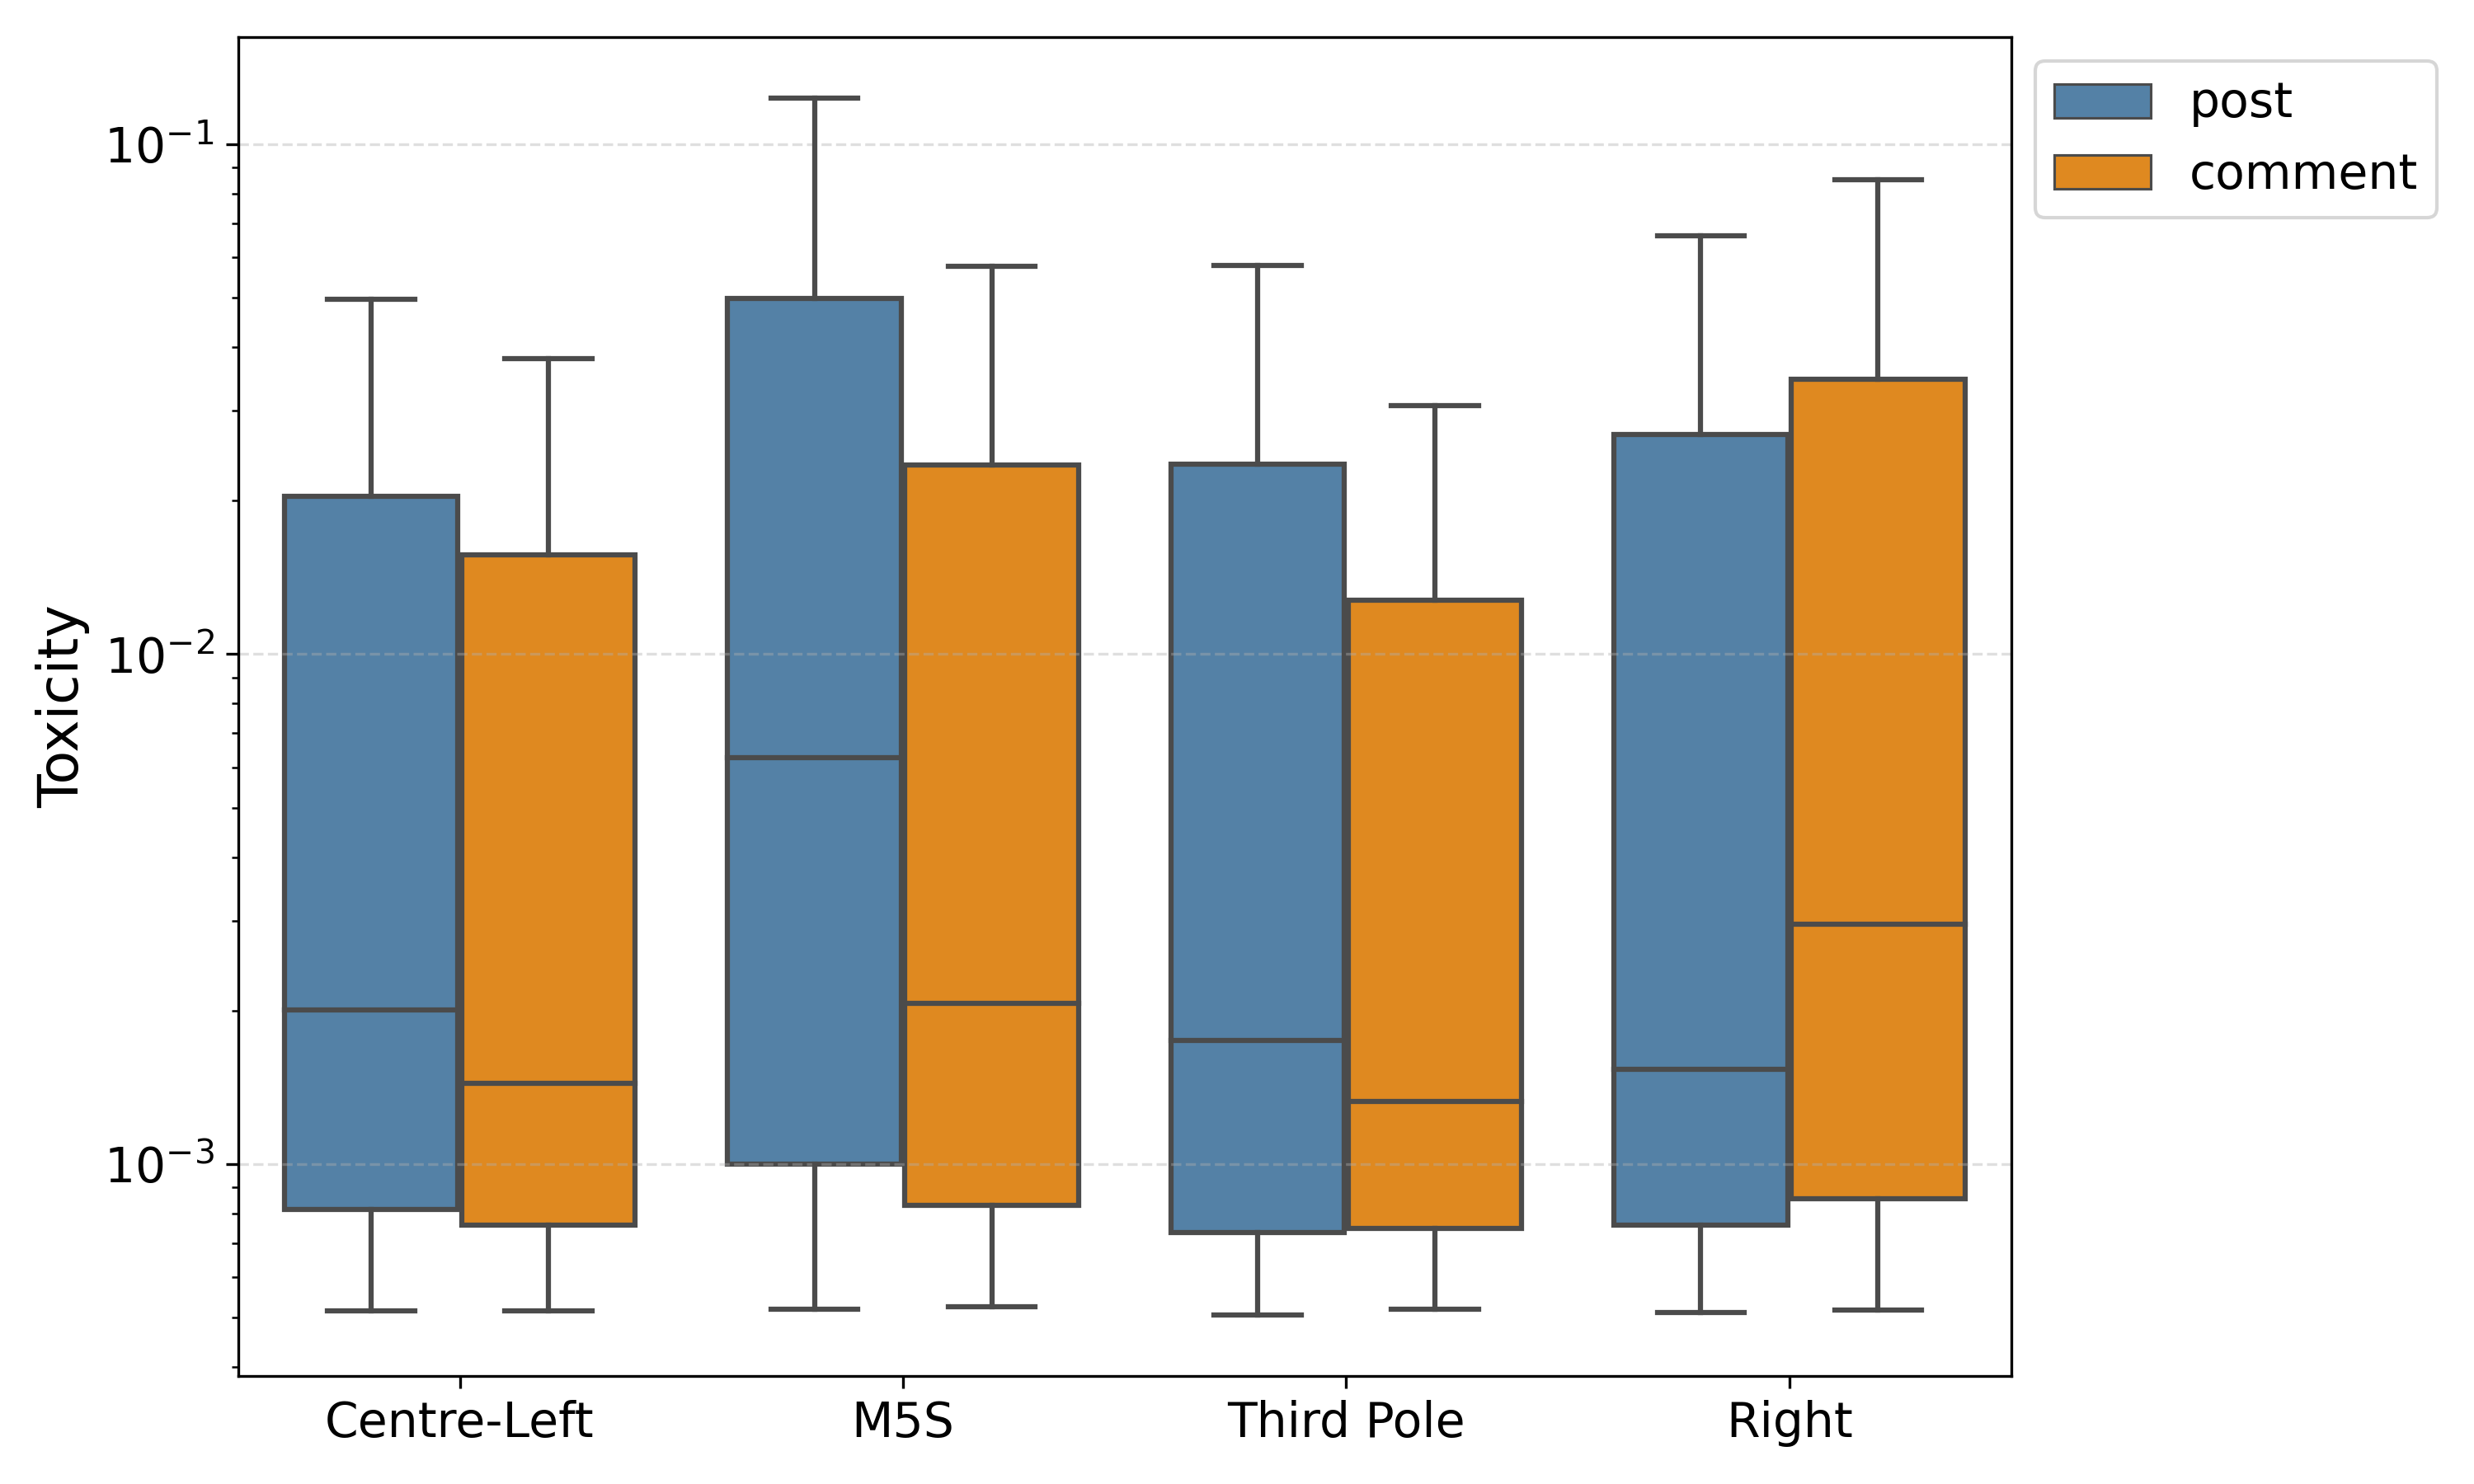
\includegraphics[width=1\linewidth]{Images/Toxicity/box_posts_vs_comments.png}
    \caption{Toxicity of LLM-generated texts.}
    \label{fig:toxicity_box}
\end{figure}


\subsection{Content recommendations}
The comparison on the two content recommendation algorithms doesn't reveal any significant behavioral difference.
At the beginning of the simulation, agents are not yet connected, so the default algorithm, \textit{ReverseChronoFollowersPopularity}, doesn't have follower information, and ends up behaving as the random recommender, \textit{ContentRecSys}.

As shown in Figure \ref{fig:recsys_comparison}, both the volume and the in-group ration of interactions is similar across the two algorithms.
To observe more meaningful effects, simulations should either run for a longer virtual time or start from a network with preexisting connections, allowing the recommender system to have a greater influence.


\begin{figure}[h]
    \centering
    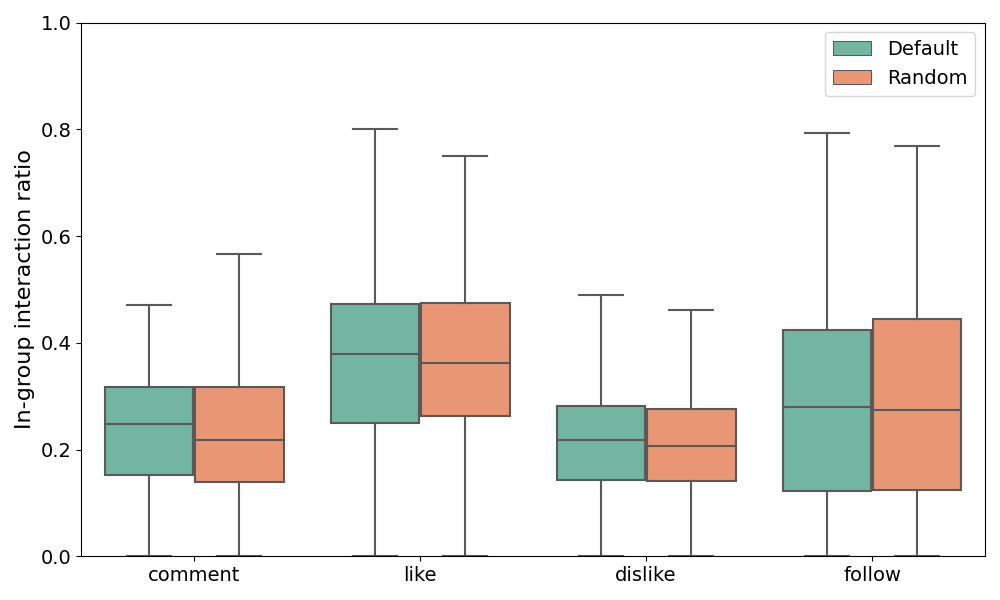
\includegraphics[width=1\linewidth]{Images/Recsys/recsys_in_group_ratio.png}
    \caption{In-group interaction ratio for the different interactions, comparing two content recommendation algorithms.}
    \label{fig:recsys_comparison}
\end{figure}